\clearpage
\section{Implementasi Fitur Bonus}
\label{sec:fitur_bonus}

Tim juga mengimplementasikan dan memverifikasi ketiga fitur bonus Milestone~2 pada kluster 3-node.

\subsection{Node pada Host Fisik Berbeda}
Ketiga node kluster (\texttt{aqua}, \texttt{ruby}, \texttt{akane}) berjalan sebagai VM QEMU/KVM berkernel terpisah pada tiga host fisik berbeda (\texttt{nexus}, \texttt{runner-1}, \texttt{runner-2}) bersama host pendukung \texttt{mainframe} dan \texttt{langley} (Tabel~\ref{tab:deklarasi_lingkungan}). Pemisahan ini memungkinkan uji partisi jaringan 35~detik (\texttt{iptables DROP} pada \texttt{akane}) dan pemadaman penuh (\textit{wipe-node} \texttt{ruby}) dengan konvergensi 100\% (\texttt{partial: false}) pascapemulihan.

\subsection{Komponen AI-Native Non-Blocking (AI Situation Summarizer)}
Layanan \texttt{summarizer-consumer} (port \texttt{8087}, \texttt{128Mi}/\texttt{256Mi}) menyusun ringkasan situasional berbasis LLM secara asinkron di luar jalur peringatan darurat (Gambar~\ref{fig:bonus_summarizer}).
\begin{enumerate}
    \item \textbf{Konsumsi Non-Blocking:} Mengonsumsi \texttt{bnpb.hazard-events} dan \texttt{bnpb.field-reports} dengan jendela geser 200~event terbaru, melakukan \textit{commit offset} segera, serta memicu perangkuman asinkron berkoalesensi (interval min. 15~detik).
    \item \textbf{Inferensi Lokal \& Proteksi:} Mengirim permintaan ke \texttt{llama-server} lokal di \texttt{langley} (\texttt{qwen3.5:9b}) dengan batas kuota 12~panggilan/menit, \textit{timeout} 30~detik, serta \textit{circuit breaker} (3~kegagalan, \textit{cooldown} 45~detik).
    \item \textbf{Validasi \& \textit{Extractive Fallback}:} Memvalidasi panjang keluaran ($\le 1.200$~karakter) dan keterkaitan \textit{grounding} terhadap kejadian aktif; bila LLM bermasalah atau gagal validasi, sistem menerbitkan ringkasan deterministik (\texttt{extractive-fallback}, \texttt{degraded: true}) via \texttt{GET /summaries} dan \texttt{/summaries/latest} (\textit{ring buffer} 30~item) beserta label \texttt{generated: true} dan \textit{disclaimer}.
\end{enumerate}
Pada pengujian langsung di kluster, \texttt{/summaries/latest} mencatat 83~sukses LLM (\texttt{qwen3.5:9b}, \textit{circuit} \texttt{closed}, latensi terakhir 7.344~ms) dan 1~\textit{fallback} tanpa menghambat \texttt{aggregator} maupun \texttt{notifier-consumer} (Gambar~\ref{fig:p5_grafana_queue}).

\begin{figure}[htbp]
    \centering
    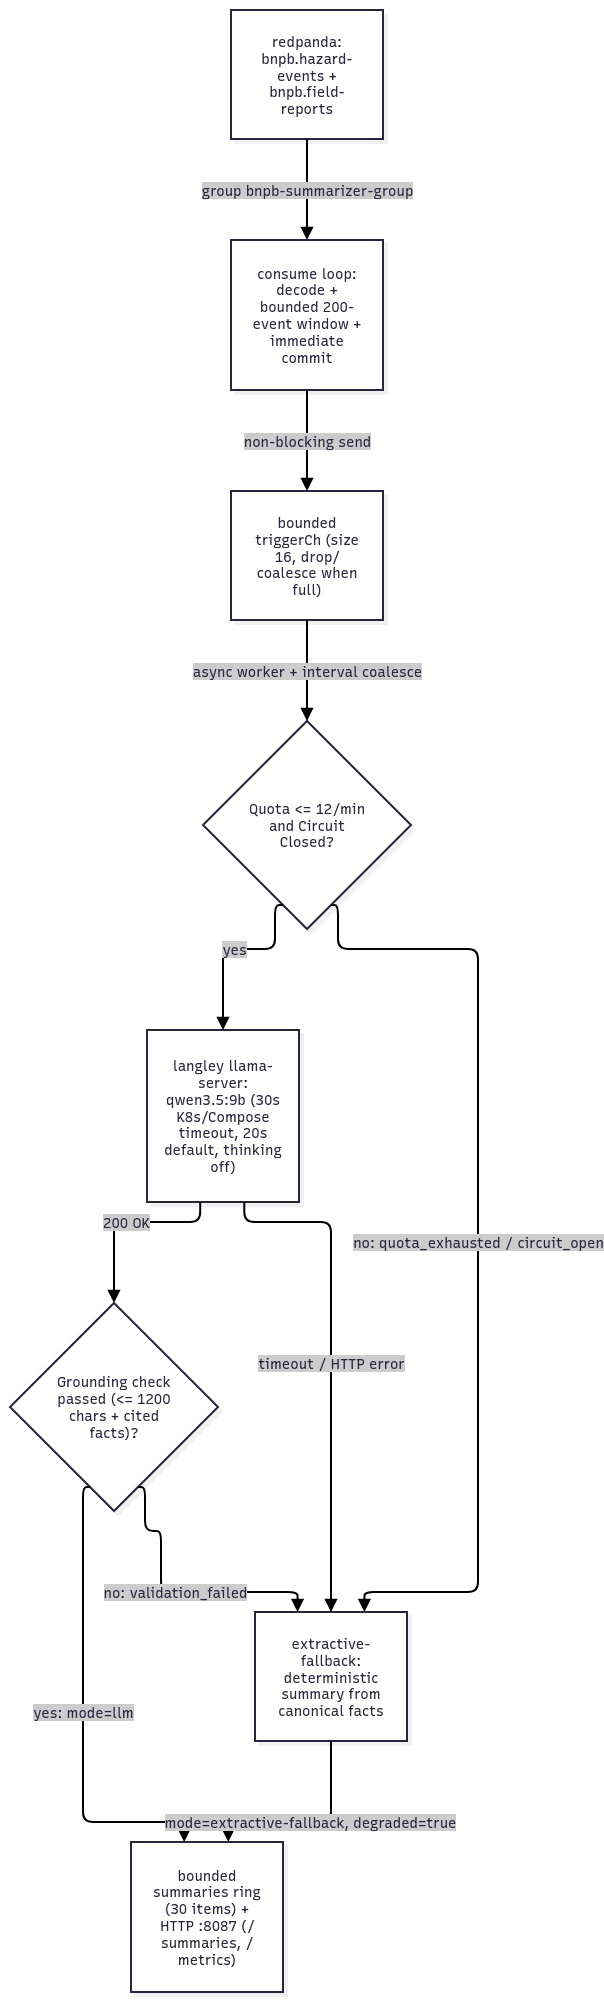
\includegraphics[height=0.76\textheight, keepaspectratio]{figures/summarizer.drawio.png}
    \caption{Arsitektur \textit{Non-Blocking AI Situation Summarizer} dengan Pembatas Kuota, \textit{Circuit Breaker}, Validasi \textit{Grounding}, dan \textit{Extractive Fallback}.}
    \label{fig:bonus_summarizer}
\end{figure}

\subsection{Kapasitas yang Menyesuaikan Diri (Horizontal Pod Autoscaler)}
Manifes \path{k8s/base/autoscaling.yaml} menerapkan penskalaan otomatis (\texttt{autoscaling/v2}, target utilisasi CPU 70\%) pada dua layanan \textit{stateless} di jalur permintaan berikut.
\begin{itemize}
    \item \textbf{\texttt{hpa/client-api}:} Rentang \texttt{2--6}~replika (CPU request \texttt{100m}) dengan jendela stabilisasi penurunan 120~detik.
    \item \textbf{\texttt{hpa/aggregator}:} Rentang \texttt{3--5}~replika untuk menjaga batas minimum HA (CPU request \texttt{250m}) dengan jendela stabilisasi penurunan 180~detik. Layanan \texttt{auth} (sesi lokal memori) dan para konsumen Kafka (3~partisi topik) sengaja tidak di-HPA.
\end{itemize}
Pengujian beban di kluster memverifikasi \textit{scale-up} otomatis (\texttt{client-api} \texttt{2 -> 4} pod pada 83\% CPU dan \texttt{aggregator} \texttt{3 -> 4} pod pada 90\% CPU) serta \textit{scale-down} otomatis pasca-stabilisasi 120~detik (\texttt{client-api} \texttt{2 -> 3 -> 2} pod tanpa memutus permintaan aktif).
